%%%%%%%%%%%%%%%%%%%%%%%%%%%%%%%%%%%%%%%%%
% Beamer Presentation
% LaTeX Template

\documentclass{beamer}
\mode<presentation> {
\usetheme{Warsaw}
}

\usepackage{multicol}
\usepackage[russian]{babel}
\usepackage{graphicx} 
\usepackage{hyperref}

\title[Introduction to Python]{Regular expressions \& Debug \& other tools} 
\author{Sugarkhuu Radnaa} 
\institute[]
{
Py4Econ in Ulaanbaatar \\ 
\medskip
\textit{py4econ@gmail.com} 
}
\date{}  % 

\begin{document}

\begin{frame}
\titlepage % Print the title page as the first slide
\end{frame}

\begin{frame}
    \frametitle{Week 7: Learning objectives}
    Get to know: 
    \begin{enumerate}
            \item Regular expressions
            \item Debugging
            \item Exception handling         
    \end{enumerate}
\end{frame}

%------------------------------------------------
% \section{Data types and structures} 
%------------------------------------------------

\begin{frame}
    \frametitle{Regular expressions}
Search "pattern"  from text and do an action
Package “re”:
    \begin{itemize}
        \item compile
        \item findall – find all matches
        \item match – match at the beginning of string
        \item search – first match anywhere in string
        \item split – split string into pieces at pattern points
        \item sub – replace match by user input
        \item group 
        \item special characters
    \end{itemize}
\end{frame}

\begin{frame}
    \frametitle{Regular expressions special characters}
            \centering
            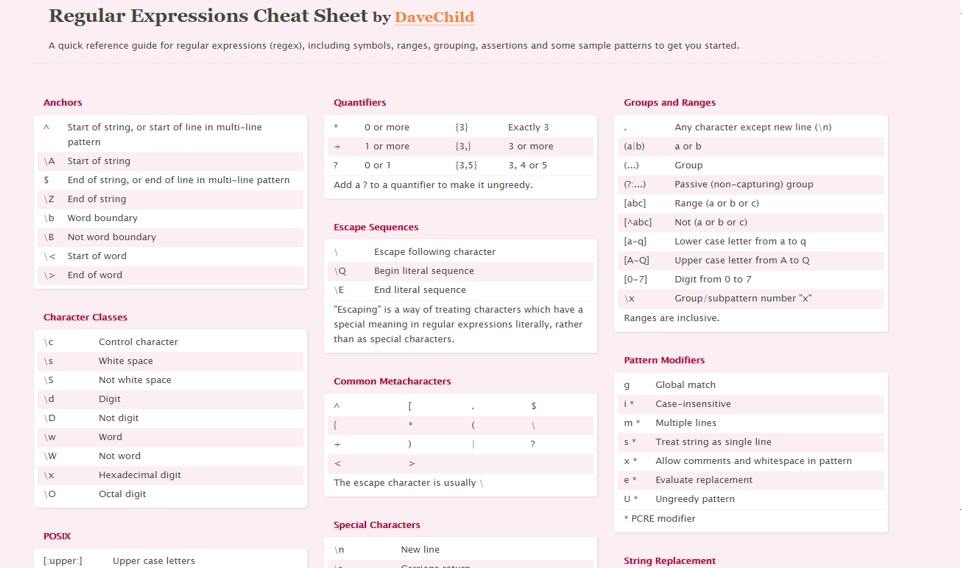
\includegraphics[scale=0.5]{figures/regex.jpg}
\end{frame}

\begin{frame}
    \frametitle{Debugging}

In IDEs (VSCode):

    \begin{itemize}
        \item Actions at breakpoints: continue, step over, step into, step out
        \item Additional actions at breakpoints - expression, hit count, log message
        \item Watch
        \item Exceptions
    \end{itemize}

\vskip 2mm

Hand inputted breakpoint:

    \begin{itemize}
        \item import pdb, pdb.set\_trace()
    \end{itemize}
\end{frame}

\begin{frame}
    \frametitle{Exception handling}
    Exceptions occur from time to time in any sort of job. 
    If you know what kind of errors potentially could occur
    and implement “remedy(ies)” on it beforehand
        \begin{center}
            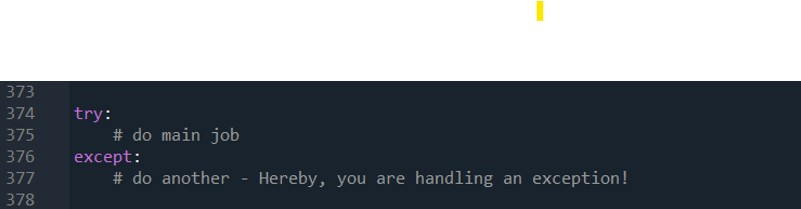
\includegraphics[scale=0.5]{figures/exception.jpg}
        \end{center}
\end{frame}

%------------------------------------------------
\section{Homework} 
%------------------------------------------------

\begin{frame}
    \frametitle{Homework}
    \begin{enumerate}
        \item Task 1
        \item Task 2
        \item Task 3
    \end{enumerate}

    \vskip 2mm
    \begin{itemize}
        \item Submit your result as a Github repository
        \item Deadline: 1 week %15 January, 2022
    \end{itemize}

\end{frame}

\begin{frame}
    \frametitle{Task 1: Regex}
    Өөрөө зохиох эсвэл бэлэн текст интернетээс олж regex-ийн 
    дараах үйлдлүүдийг ашиглан текстүүд гаргаж авах жишээнүүд үзүүл 
    (нэг бүр дээр нь бус хамтад нь ашиглаж болно. Гэхдээ доорх бүх тэмдгээс ядаж 1 удаа ашиглаарай)

    \begin{itemize}
        \item {[a-zA-Z0-9], [a-z],[A-Z],[0-9]}
        \item \textbackslash d, \textbackslash D, \textbackslash w, \textbackslash W, \textbackslash s
        \item \^{}, \$, ?, *, +, .
        \item \{m,n\}, \{,n\}, \{m,\}, \{n\}
        \item Look behind, Look ahead, Negative look behind, Negative look ahead
    \end{itemize}
\end{frame}

\begin{frame}
    \frametitle{Task 2: Exception}
    \begin{enumerate}
        \item Generate array of 1000 random integers in numpy and create an array with only the negative even numbers.
        \item Loop one by one through this array …
        \item \ldots when negative & odd, then raise “odd error” and continue to next loop, 
        \item \ldots when even but positive, raise “sign error” and continue to next loop \ldots
        \item \ldots when “negative even”, then append your list. 
    \end{enumerate}
\end{frame}

\begin{frame}
    \frametitle{Task 3: Debugging}
    \begin{itemize}
        \item Debugging гэж юу вэ?
        \item Breakpoint – ийн ямар 3 төрөл (log message г.м) Vscode дээр байдаг вэ?
        \item Debug-ийн step into, step over, stop out – ийн ялгааг тайлбарла 
    \end{itemize}
\end{frame}



\begin{frame}
\Huge{\centerline{Thank you!}}
\end{frame}

%----------------------------------------------------------------------------------------

\end{document} 